\documentclass[../main.tex]{subfiles}
\begin{document}
    \chapter{Research Method}\label{ch:research_method}

    In this research we will try to answer research questions.
    Section \ref{sec:research_question} describes the research questions.
    In section \ref{sec:types} we will explain more about types, subtypes and their relationship.
    Section \ref{sec:research_context} explains in which context the research is executed.

    \section{Research question}\label{sec:research_question}
    The main research question we want to answer is:
    \\
    \begin{quote}
        Will the use of annotations\footnotemark{} help to do better static source code analysis?
        \footnotetext{The annotations are limited to: \texttt{@param}, \texttt{@return}, \texttt{@var}, and \texttt{@inheritDoc}.}
    \end{quote}
    Subquestions:
    \begin{quote}
        - What is the accuracy (recall and precision) of our analysis?
        \\
        - Are annotations used in programs reliable?
    \end{quote}
    The subquestions are here to support the main question. 
    In the first question we want to measure the precision and recall of this research.
    With precision we want to measure if the results we have are reliable.
    With recall we want to have the number of results we were able to reveal.
    \\
    In the second subquestion we want to know if the annotations conform to the documentation.
    We will measure this by doing the analysis without using annotations, and see if the results fit the annotations.    
    
   \section{Types}\label{sec:types}
    PHP is dynamically typed and allow coercions and duck-typing.
    Coercion make it possible for variables to hold different types
    Duck-typing checks the object instead of the class.
    
    \begin{rascal}
\CAT{Keyword}{module} lang::php::m3::TypeSymbol

\CAT{Keyword}{data} TypeSymbol
  = \textbackslash{}any()        | array(TypeSymbol arrayType)
  | boolean()     | class(\CAT{Keyword}{loc} decl)
  | float()       | integer()
  | null()        | object()
  | resource()    | string()
  ;
    \end{rascal}
    
    \subsection{PHP types}
    PHP has a similar class inheritance structure and interface implementation as Java.
    The main difference is that in PHP all class are \texttt{public} and that inner classes are not allowed in PHP. 
    \\
    The basis types in PHP are integers, floats (similar to doubles and reals), booleans, strings, arrays, resources and null.
    When variables are initialised without a values, they are null. The recourse type is a special one which is not important for this research.
 
    \subsection{Subtypes}
    
    Explain something about subtypes here. For now, only this figure\ref{fig:subtypeTree}

    \begin{figure}[H]
        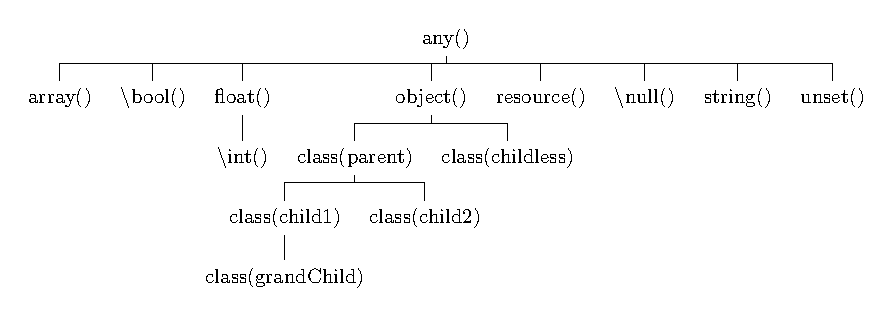
\includegraphics{Diagrams/Subtypes.pdf}
        \caption{Subtype hierarchy}
        \label{fig:subtypeTree}
    \end{figure}

    The subtype relation of class inheritance is a \gls{reflexive transitive closure} relation.
    A class extension of \textbf{\texttt{class A}} on \textbf{\texttt{class C}} will define \textbf{\texttt{class A}} as a subtype of \textbf{\texttt{class C}} in our analysis, as you can see in figure \ref{fig:subtypes}.
    If a class does not extend another class, it will implicitly extend the \gls{stdClass} class.
    You can see that this happens with \textbf{\texttt{class D}} in the example.
    The \textbf{\texttt{stdClass}} is represented as the type \textbf{\texttt{object()}} in our analysis.
    \\
    The basic PHP types also contain a subtype relation.
    Integers are subtypes of floats.
 
    % show three images next to each other
    \begin{figure}[H]
    \begin{subfigure}[b]{.33\textwidth}
      \begin{center}
      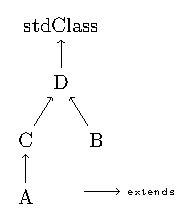
\includegraphics[scale=1]{Diagrams/Inheritance_example.pdf}
      \caption{Inheritance relation}
      \label{fig:subtype}
      \end{center}
    \end{subfigure}
    \begin{subfigure}[b]{.33\textwidth}
      \begin{center}
      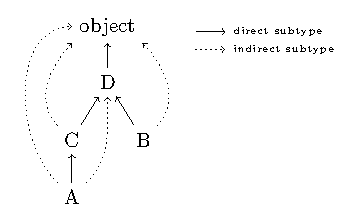
\includegraphics[scale=1]{Diagrams/Subtypes_example.pdf}
      \caption{Subtype relation}
      \label{subtype_tc}
      \end{center}
    \end{subfigure}
    \begin{subfigure}[b]{.33\textwidth}
      \begin{center}
      \lstinputlisting[nolol=true,xleftmargin=20pt,xrightmargin=20pt,language=PHP]{src/php/inheritance.php}
      \caption{Inheritance in PHP}
      \label{subtype_code}
      \end{center}
    \end{subfigure}
    \caption{Relation of subtypes among classes}
    \label{fig:subtypes}
    \end{figure}

    \section{Research context}\label{sec:research_context}
    In order to let our research take place, we need to make sure that some environment variables are constant.
    
    \paragraph{Program Correctness}
    In order to be able to execute this research we will need to assume that the program is correct and works as intended. 
    We will assume that the system contains no bugs.
    This is needed to be able to say something about the programs we analyse.
    
    \paragraph{File includes}
    In this research we will assume that all file are included during runtime. 
    When a PHP system is constructed of classes with namespaces, the files will be logically loaded using PHP's autoloader.
    Because most recent systems use namespaces, we will assume that all files are included.
    For legacy systems, this can influence the results of this research.
    
    \paragraph{Register globals}
    Register globals allows variables to be magically be created from GET and POST values.
    Since it is discouraged to use this setting, we will assume that all software products have this setting disabled.
    
    \paragraph{PHP Warnings}
    For this research we will ignore all warnings.
    Warnings do not alter the behaviour of the program.
    In a normal production environment, the warnings are not shown.
    
    \paragraph{Sensitivity}
    Our analysis is flow-, control-, and context-insensitive.
    Flow-insensitive means that we do not look at messages between objects, and only look in the body of a method.
    Control-insensitive means that we ignore all control structures. 
    Examples of control structures are \texttt{if}, \texttt{else}, and \texttt{switch}.
    Context-insensitive means that we do not look at the order of which code is executed.
     
    
\end{document}
